\documentclass[10pt,letterpaper]{article}
\usepackage[margin=0.72in,headheight=14pt]{geometry}
\usepackage[T1]{fontenc}
\usepackage{newtxtext,newtxmath}
\usepackage{amsmath,booktabs,array,xcolor,tikz,fancyhdr}
\usetikzlibrary{arrows.meta,positioning}
\usepackage[colorlinks=true,linkcolor=teal,urlcolor=teal]{hyperref}
\hypersetup{pdftitle={The mathematics of the implemented shifted short recurrence},pdfauthor={Implementation note},pdfsubject={Fortran PMINRES and custom PETSc shifted Lanczos recurrence}}
\definecolor{ink}{HTML}{16324F}
\definecolor{pale}{HTML}{EDF4F7}
\setlength{\parindent}{0pt}
\setlength{\parskip}{5pt}
\setlength{\abovedisplayskip}{7pt}
\setlength{\belowdisplayskip}{7pt}
\pagestyle{fancy}\fancyhf{}
\fancyhead[L]{\small\color{ink}Shifted Lanczos recurrence}
\fancyhead[R]{\small Implementation note\enspace /\enspace 5 October 2026}
\fancyfoot[L]{\small Fortran PMINRES and its PETSc port}
\fancyfoot[R]{\small\thepage\ / 3}
\renewcommand{\headrulewidth}{0.3pt}
\newcommand{\norm}[1]{\left\lVert #1\right\rVert_2}
\newcommand{\adj}{^{\dagger}}
\newcommand{\sect}[1]{\vspace{5pt}{\large\bfseries\color{ink}#1}\par}
\newcommand{\code}[1]{\texttt{#1}}
\begin{document}
{\LARGE\bfseries\color{ink}The mathematics of the implemented\par shifted short recurrence}\par
\vspace{3pt}
{\large One algorithm, two implementations, and a crucial residual distinction}

This note describes the actual updates in \code{src/linsys.f90} and
\code{petsc\_shifted\_pminres.c}. The C routine is a custom PETSc port, not
PETSc's built-in \code{KSPMINRES}. The derivation below assumes exact arithmetic
and no breakdown; the last page explains the practical stopping checks.

\sect{1. The structure that makes a short recurrence possible}
We solve, with no preconditioner and initial guess $x_0=0$,
\begin{equation}
 Ax=b,\qquad A=H+i\gamma I,\qquad H=H\adj,\quad \gamma\in\mathbb R.
 \label{eq:system}
\end{equation}
A real energy shift can be absorbed into $H$. For $\gamma\ne0$, $A$ is generally
\emph{not Hermitian}, but it is normal:
$A\adj A=AA\adj=H^2+\gamma^2 I$.
Also $\mathcal K_k(A,b)=\mathcal K_k(H,b)$, since adding a scalar multiple of
$I$ does not change the Krylov subspace. Thus the basis can be generated by
Hermitian Lanczos even though the projected diagonal is complex.

Set $\beta_1=\norm b$, $v_1=b/\beta_1$, and $v_0=0$ (handle $b=0$ separately).
At iteration $j$, compute
\begin{align}
 q_j&=Av_j, & \alpha_j&=v_j\adj q_j,\notag\\
 t_j&=q_j-\alpha_jv_j-\beta_jv_{j-1}, &
 \beta_{j+1}&=\norm{t_j},\qquad v_{j+1}=t_j/\beta_{j+1}. \label{eq:lanczos}
\end{align}
Here $\alpha_j=v_j\adj Hv_j+i\gamma$. Consequently the imaginary shift cancels
in $q_j-\alpha_jv_j$, leaving exactly the Hermitian Lanczos basis recurrence.
For $j=1$, the arbitrary-looking use of $\beta_1$ as a coupling is harmless
because $v_0=0$. In exact arithmetic the $v_j$ are orthonormal.

\sect{2. A large sparse problem becomes a small tridiagonal one}
Let $V_k=[v_1,\ldots,v_k]$. The recurrence gives
\begin{equation}
 AV_k=V_{k+1}\underline T_k,\qquad
 \underline T_k=
 \begin{bmatrix}
 \alpha_1&\beta_2&&\\
 \beta_2&\alpha_2&\ddots&\\
 &\ddots&\ddots&\beta_k\\
 &&\beta_k&\alpha_k\\
 &&&\beta_{k+1}
 \end{bmatrix}_{(k+1)\times k}.
 \label{eq:projection}
\end{equation}
For $x_k=V_ky_k$, $b-Ax_k=V_{k+1}(\beta_1e_1-\underline T_ky_k)$.
The next page shows how the code updates $x_k$ without storing $V_k$ or
explicitly forming this small matrix.

\begin{center}
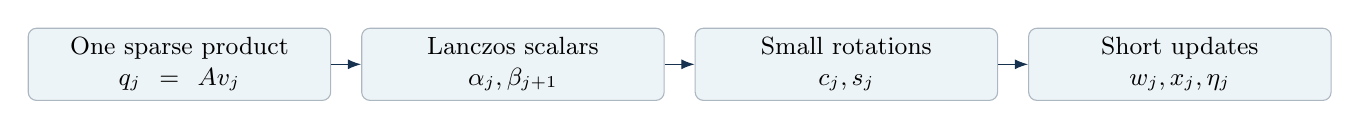
\begin{tikzpicture}[node distance=0.38cm,box/.style={draw=ink!35,fill=pale,rounded corners=3pt,align=center,minimum height=0.70cm,font=\small},>=Latex]
\node[box,text width=1.42in] (a) {One sparse product\\$q_j=Av_j$};
\node[box,text width=1.42in,right=of a] (b) {Lanczos scalars\\$\alpha_j,\beta_{j+1}$};
\node[box,text width=1.42in,right=of b] (c) {Small rotations\\$c_j,s_j$};
\node[box,text width=1.42in,right=of c] (d) {Short updates\\$w_j,x_j,\eta_j$};
\draw[->,ink] (a)--(b);\draw[->,ink] (b)--(c);\draw[->,ink] (c)--(d);
\end{tikzpicture}
\end{center}

\newpage
\sect{3. The scalar and solution recurrences, exactly as coded}
Use $c_0=c_{-1}=1$, $s_0=s_{-1}=0$, $w_0=w_{-1}=0$, and
$\eta_0=\widehat r_0=\beta_1$. After obtaining $\alpha_j$ and $\beta_{j+1}$,
the code applies
\begin{align}
 \delta_j &= c_{j-1}\alpha_j-c_{j-2}s_{j-1}\beta_j,\notag\\
 d_j &= \sqrt{\delta_j^{\,2}+\beta_{j+1}^{\,2}},\notag\\
 u_j &= s_{j-1}\alpha_j+c_{j-2}c_{j-1}\beta_j,
 & z_j &= s_{j-2}\beta_j,\label{eq:scalars}\\
 c_j &= \delta_j/d_j, & s_j &= \beta_{j+1}/d_j.\notag
\end{align}
The square root is a \emph{complex} square root. In particular the code uses
$\delta_j^2$, not $|\delta_j|^2$. With $d_j\ne0$, the update is
\begin{align}
 w_j &= \frac{v_j-u_jw_{j-1}-z_jw_{j-2}}{d_j},\label{eq:w}\\
 x_j &= x_{j-1}+c_j\eta_{j-1}w_j,\label{eq:x}\\
 \eta_j&=-s_j\eta_{j-1}, &
 \widehat r_j&=|s_j|\widehat r_{j-1}=|\eta_j|.\label{eq:estimate}
\end{align}
The two stored Lanczos arrays alternate roles. The current array initially
holds $\beta_jv_j$ and is normalized to $v_j$; the old array holds $v_{j-1}$.
Multiplying the old array by $\beta_j$ therefore produces the last term in
Eq.~\eqref{eq:lanczos}. The newly written array is $t_j=\beta_{j+1}v_{j+1}$.

\sect{4. Why these updates correspond to elimination}
The local transformation is
\begin{equation}
 G_j=\begin{bmatrix}c_j&s_j\\-s_j&c_j\end{bmatrix},\qquad
 G_j\begin{bmatrix}\delta_j\\\beta_{j+1}\end{bmatrix}
 =\begin{bmatrix}d_j\\0\end{bmatrix},\qquad G_j^T G_j=I.
 \label{eq:rotation}
\end{equation}
Embedding these rotations in successive row pairs gives
$Q_k\underline T_k=\begin{bmatrix}R_k\\0\end{bmatrix}$.
$R_k$ has only a diagonal and two superdiagonals: in column $j$, its nonzero
entries are $z_j,u_j,d_j$. If $W_k=V_kR_k^{-1}$, equating column $j$ in
$W_kR_k=V_k$ gives Eq.~\eqref{eq:w}. The transformed RHS has newly fixed
entry $c_j\eta_{j-1}$ and remaining entry $\eta_j$, yielding Eq.~\eqref{eq:x}.

\colorbox{pale}{\parbox{\dimexpr\linewidth-2\fboxsep\relax}{\textbf{Important distinction.}
These rotations are complex-orthogonal ($G_j^TG_j=I$), but generally not
unitary ($G_j\adj G_j\ne I$). Therefore this elimination is not, in general,
a Euclidean minimum-residual solve. The name \code{pminres\_csr} should not
be read as a guarantee that $\norm{b-Ax_j}$ is minimized over the Krylov subspace.}}

\sect{5. Mapping the notation to the source}
\small
\begin{tabular}{@{}p{1.30in}p{2.42in}p{2.52in}@{}}
\toprule
Mathematics & Fortran & PETSc C port\\\midrule
$\beta_j,\beta_{j+1}$ & \code{beta0, beta1} & \code{beta, next}\\
$c_{j-1},c_{j-2}$ & \code{gamma0, gamma1} (before update) & same names\\
$s_{j-1},s_{j-2}$ & \code{sigma0, sigma1} (before update) & same names\\
$d_j,u_j,z_j$ & \code{rho1, rho2, rho3} & same names\\
$\eta_j,\widehat r_j$ & \code{eta, res} & \code{eta, estimate}\\
\bottomrule
\end{tabular}\par
\normalsize
The rotation variables named \code{gamma0/gamma1} are \emph{not} the physical
broadening $\gamma$ in Eq.~\eqref{eq:system}.

\newpage
\sect{6. Why the true residual must be checked}
After solving the first $k$ transformed equations, the projected residual is
$Q_k^T e_{k+1}\eta_k$. Thus, while the Lanczos basis remains orthonormal,
\begin{equation}
 \boxed{\norm{b-Ax_k}=|\eta_k|\,\norm{Q_k^T e_{k+1}}.}
 \label{eq:true}
\end{equation}
The code tracks only $\widehat r_k=|\eta_k|$.
The missing factor need not be one for complex-orthogonal rotations.
Loss of Lanczos orthogonality and accumulated roundoff can further separate
the estimate from the actual residual. Their disagreement is therefore
\emph{not only a floating-point effect}.

\textbf{A two-dimensional example.}
Take $H=\operatorname{diag}(-1,1)$, $\gamma=0.2$, and
$b=(1,1)^T/\sqrt2$. Then $\beta_1=1$, $\alpha_1=0.2i$,
$\beta_2=1$, $d_1=\sqrt{0.96}$,
$c_1=0.2i/\sqrt{0.96}$, and $s_1=1/\sqrt{0.96}$.
The implemented first step gives
\begin{equation}
 x_1=\frac{0.2i}{0.96}b,\qquad
 \widehat r_1=1.020621,\qquad
 \norm{b-Ax_1}=|s_1|\sqrt{|s_1|^2+|c_1|^2}=1.062296.
 \label{eq:example}
\end{equation}
By contrast, minimizing $\norm{b-tAb}$ over complex $t$ gives
$t=-0.2i/1.04$. This illustrates why the implemented shifted recurrence
must not be identified with standard Euclidean MINRES.

\textbf{Actual stopping behavior.}
Fortran stops when $\widehat r_k\le\tau$ (or at its iteration cap), then prints
$\norm{Ax_k-b}$; that final check does not change its always-zero \code{info}.
The PETSc port recomputes the true residual when the estimate first qualifies
(and on zero next-Lanczos norm), and accepts convergence only if
$\norm{Ax_k-b}\le\tau$. Otherwise it continues or reports breakdown/iteration
failure. It also checks zero/nonfinite $d_j$; the production Fortran has no
corresponding explicit guard. Complex-orthogonal elimination can break down
when $\delta_j^2+\beta_{j+1}^2=0$, even if the two terms are individually nonzero.

\sect{7. Same mathematics, different distributed kernels}
Fortran's \code{dot\_product(v,q)} computes $v\adj q$, followed by an MPI sum.
PETSc's convention is \code{VecDot(x,y)} $=y\adj x$, so the equivalent call is
\code{VecDot(work,v,\&alpha)}, \emph{not} the reversed argument order.
The C update \code{VecAXPBYPCZ(z,a,b,c,x,y)} means $z\leftarrow ax+by+cz$;
it fuses the three-term vector updates above. Both implementations store five
work vectors plus the solution and normally use one matrix product and two
global scalar reductions per iteration, with extra work for residual checks.
GMRES instead stores an expanding basis and orthogonalizes against it.

For $\gamma\ne0$, a useful accuracy bound follows directly from
$A\adj A=H^2+\gamma^2I$:
$\norm{x_\star-x_k}\le\norm{b-Ax_k}/|\gamma|$.
It requires the \emph{true} residual, and becomes less favorable as broadening
shrinks. General preconditioning need not preserve the structure used here.

\vfill
{\footnotesize\color{ink}\textbf{Implementation sources and API references.}\par}
{\footnotesize
Local implementation sources (inspected 5 October 2026):\\
\code{src/linsys.f90}; \code{petsc\_shifted\_pminres.c}; adapter \code{petsc\_shifted\_pminres.py}.\\
Equations and the worked example are derived directly from these updates.
PETSc API conventions:
\href{https://petsc.org/release/manualpages/Vec/VecDot/}{VecDot documentation};
\href{https://petsc.org/release/manualpages/Vec/VecAXPBYPCZ/}{VecAXPBYPCZ documentation}.
}
\end{document}
